\documentclass[runningheads]{llncs}
\usepackage{graphicx}
\usepackage{amsmath,amssymb} % define this before the line numbering.
\usepackage{ruler}
\usepackage{color}
\usepackage{subfig}
\usepackage[width=122mm,left=12mm,paperwidth=146mm,height=193mm,top=12mm,paperheight=217mm]{geometry}
\usepackage[pagebackref=true,breaklinks=true,colorlinks,bookmarks=false]{hyperref}
\begin{document}
% \renewcommand\thelinenumber{\color[rgb]{0.2,0.5,0.8}\normalfont\sffamily\scriptsize\arabic{linenumber}\color[rgb]{0,0,0}}
% \renewcommand\makeLineNumber {\hss\thelinenumber\ \hspace{6mm} \rlap{\hskip\textwidth\ \hspace{6.5mm}\thelinenumber}}
% \linenumbers
\pagestyle{headings}

% Definitions
\newcommand{\argmax}{\operatornamewithlimits{argmax}}
\def\subsectionautorefname{section}
\definecolor{light-gray}{gray}{0.5}
\newcommand{\aside}[1]{\textcolor{light-gray}{\emph{#1}}}
\newcommand{\todo}[1]{\textcolor{red}{\emph{#1}}}
\newcommand{\cut}[1]{\textcolor{light-gray}{#1}}
\newcommand{\comment}[1]{}

\mainmatter
\def\ECCV12SubNumber{***}  % Insert your submission number here

\title{Timely Object Detection}

\titlerunning{ECCV-12 submission ID \ECCV12SubNumber}

\authorrunning{ECCV-12 submission ID \ECCV12SubNumber}

\author{Anonymous ECCV submission}
\institute{Paper ID \ECCV12SubNumber}

\maketitle

\begin{abstract}
\end{abstract}

\section{Sequential Decision Problem} \label{sec:sdp}

We first describe the requirements for our target system, and set the notation.
Details of our implementation are then given.

\subsection{Problem Setting} \label{sec:problem_setting}

We deal with a dataset of images $\mathcal{D}$, where each image $\mathcal{I}$ contains at least one, and often multiple, objects.
Each object is labeled with exactly one category label $k \in \{1, \dots, K\}$.

The multi-class, multi-label \emph{classification} problem asks whether $\mathcal{I}$ contains at least one object of class $k$.
The answer for a single label is given with a real-valued confidence by a function $\emph{classify}(\mathcal{I},k)$.
We write the ground truth for an image as $\mathbf{C}=\{C_1,\dots,C_K\}$, where $C_k \in \mathbb{B} = \{0,1\}$ is set to $1$ if an object of class $k$ is present.

The answer is evaluated by plotting precision vs. recall across dataset $\mathcal{D}$ (by progressively lowering the confidence threshold for a positive label) and integrating to yield the Average Precision (AP) metric \cite{pascal-voc-2010}.

\cut{
We can make the classification problem more difficult by posing the \emph{counting} problem, which asks how many objects of class $k$ are present in $\mathcal{I}$, for each $k$.
This setting is not commonly evaluated; we mention it for its usefulness in later exposition.
}

The \emph{detection} problem is to output a list of bounding boxes (sub-images defined by four coordinates), each with a real-valued confidence that it encloses a single instance of an object of class $k$, for each $k$.
The answer for a single class is given by an algorithm $\emph{detect}(\mathcal{I},k)$, which outputs a list of sub-image bounding boxes $B$ and their associated confidences.

To highlight the hierarchical structure of these problems, we note that (1) the confidences may be given by $\operatorname{classify}(b,k)$ for each sub-image $b \in B$; (2) the correct answer to the detection problem also answers the counting and classification problems.

The following exposition deals with the classification problem, although we evaluate performance on both the classification and detection tasks.

\subsection{Multi-class Classification Policy}

\begin{table}
\centering
\caption{Summary of our notation.}
\label{tab:notation}
\begin{tabular}{|l|l|}
	\hline
	$\mathcal{I}$	&	image \\
	$C_k$         & presence of class $k \in \{1,\dots,K\}$ \\ 
	$t$           & time into episode \\ 
	$T_s$, $T_d$  & start and deadline times \\ 
	$b^j$        	& belief state at step $j$ \\ 
	$\pi$         & policy function, $b \mapsto a \in \mathcal{A}$ \\
	$\mathcal{A}$ & set of actions $a_i \in \{\mathcal{L} \cup \mathcal{F}\}$\\ 
	$\mathcal{F}$ & set of featurization actions \\
	$\mathcal{L}$ & set of classification actions\\
	$o_i$					&	a real-valued observation upon executing $a_i \in \mathcal{L}$\\
	$\mathcal{O}$	& set of executed actions\\
	$\mathbf{o}$	& set of observations $\{o_i | a_i \in \mathcal{O}\}$\\
	$c(a_i)$				& cost of executing $a_i$, in units of $t$\\
	\hline
\end{tabular}\end{table}

\begin{figure}[h!]
\center{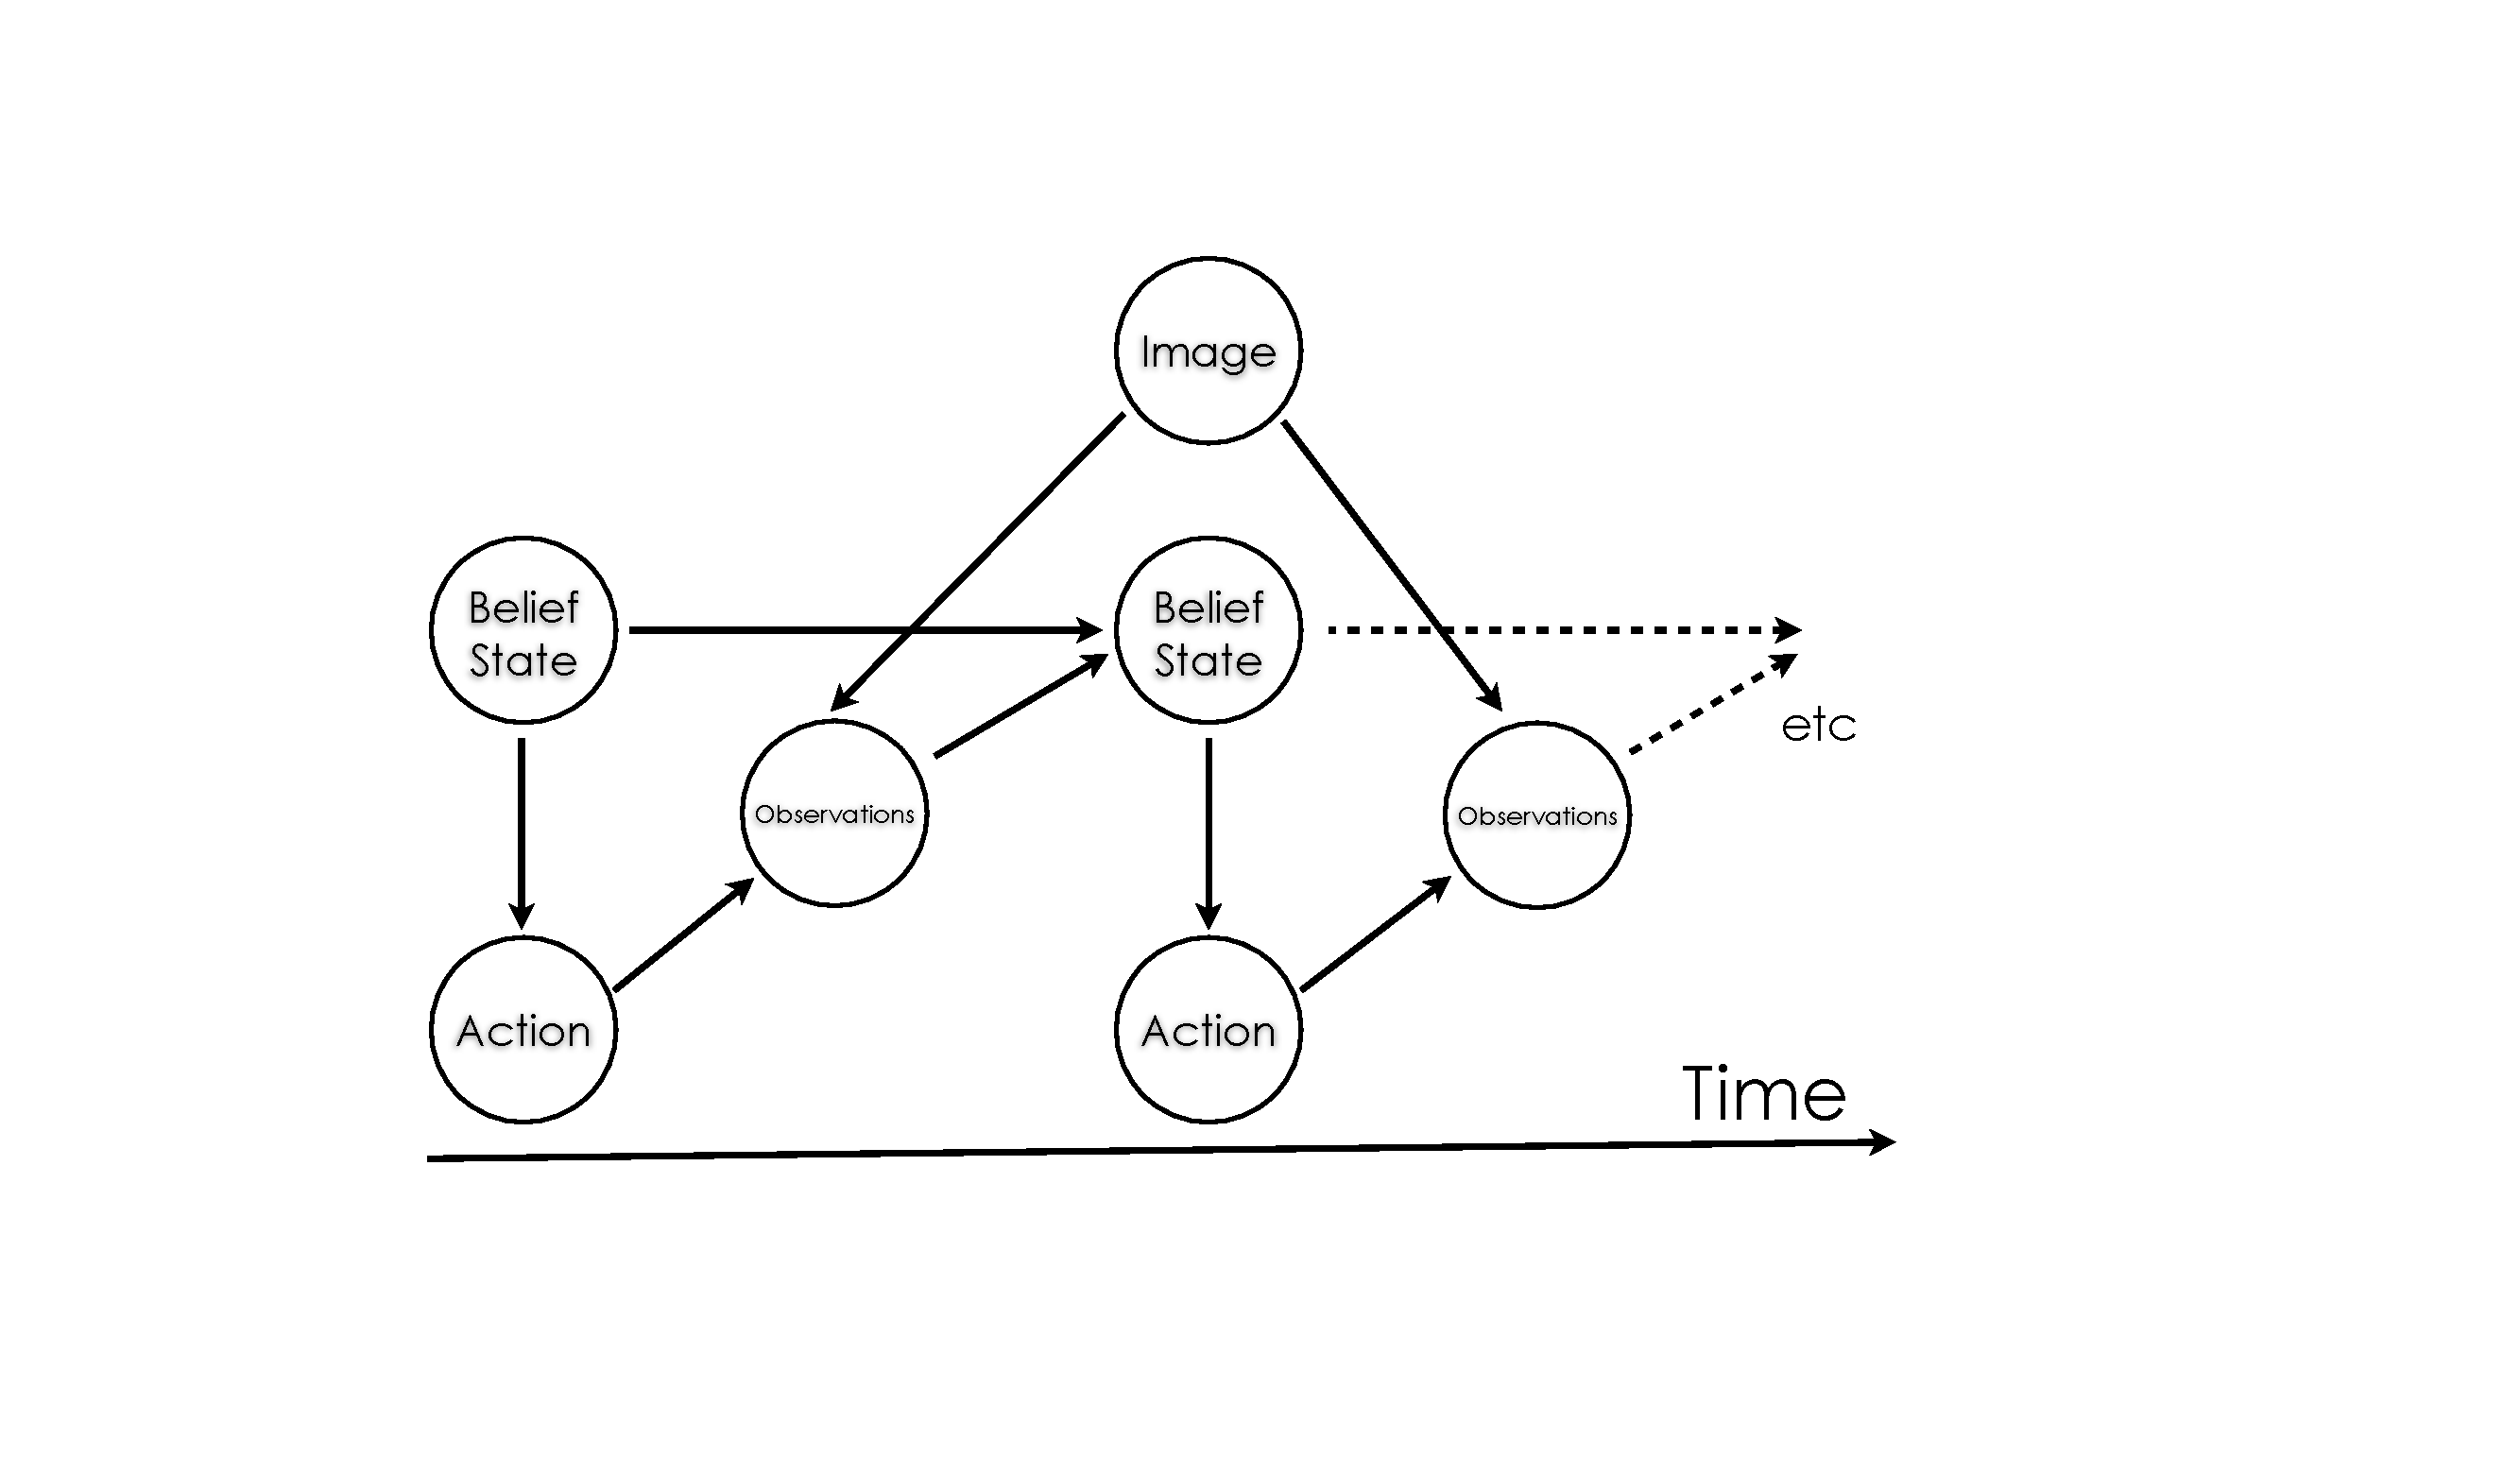
\includegraphics[width=0.66\linewidth]
    {figures/pomdp.pdf}}
  \caption{Summary of our approach to the problem. Our system has two major parts: (1) selecting an action by predicting its value; (2) updating the belief state with observations resulting from the action.}
  \label{fig:evaluation}
\end{figure}

Our goal is a multi-class classification policy $\pi$ that takes an image $\mathcal{I}$ and outputs $\{\emph{classify}(1), \dots, \emph{classify}(K)\}$.
The policy repeatedly selects an action $a_i$ from a set of actions $\mathcal{A}$, executes it, potentially receives an observation $o_i$, and selects the next action.

A dynamic, or ``closed-loop,'' policy bases action selection on observations received from previous actions, exploiting the signal in inter-object and scene context for a maximally efficient path through the actions.
This is our goal, and what sets our formulation apart from multi-class systems that evaluate in a fixed order, such as simple cascades \cite{Viola2001} or \todo{add another one}.

The set of actions $\mathcal{A}$ can include classifiers and feature computations.
For simplicity of exposition, let $\mathcal{A}$ consist of $2K+2$ actions:
\begin{itemize}
	\item $F^\text{co}$, a complex spatial pyramid (SP) featurization of the image
	\item $K$ classifiers $L^\text{co}_i$: one-vs-all SVMs trained on the SP feature
	\item $F^\text{sc}$, a quick GIST featurization of the image
	\item $K$ classifiers $L^\text{sc}_i$: one-vs-all SVMs on the GIST feature
\end{itemize}

Each classifier $L$ or feature computation $F$ has an expected cost $c(\cdot)$ of execution.
Depending on the setting, the cost can be defined in terms of algorithmic runtime analysis, an idealized property such as number of \emph{flops}, or simply the empirical runtime on specific hardware.
We take the empirical approach: every executed action advances $t$, the \emph{time into episode}, by its empirical runtime.

The system is given two times: the setup time $T_s$ and deadline $T_d$.
Between these times, the system must strive for the goal of \emph{Anytime} performance and give the best possible answer at any point.

\begin{figure}[h!]
\center{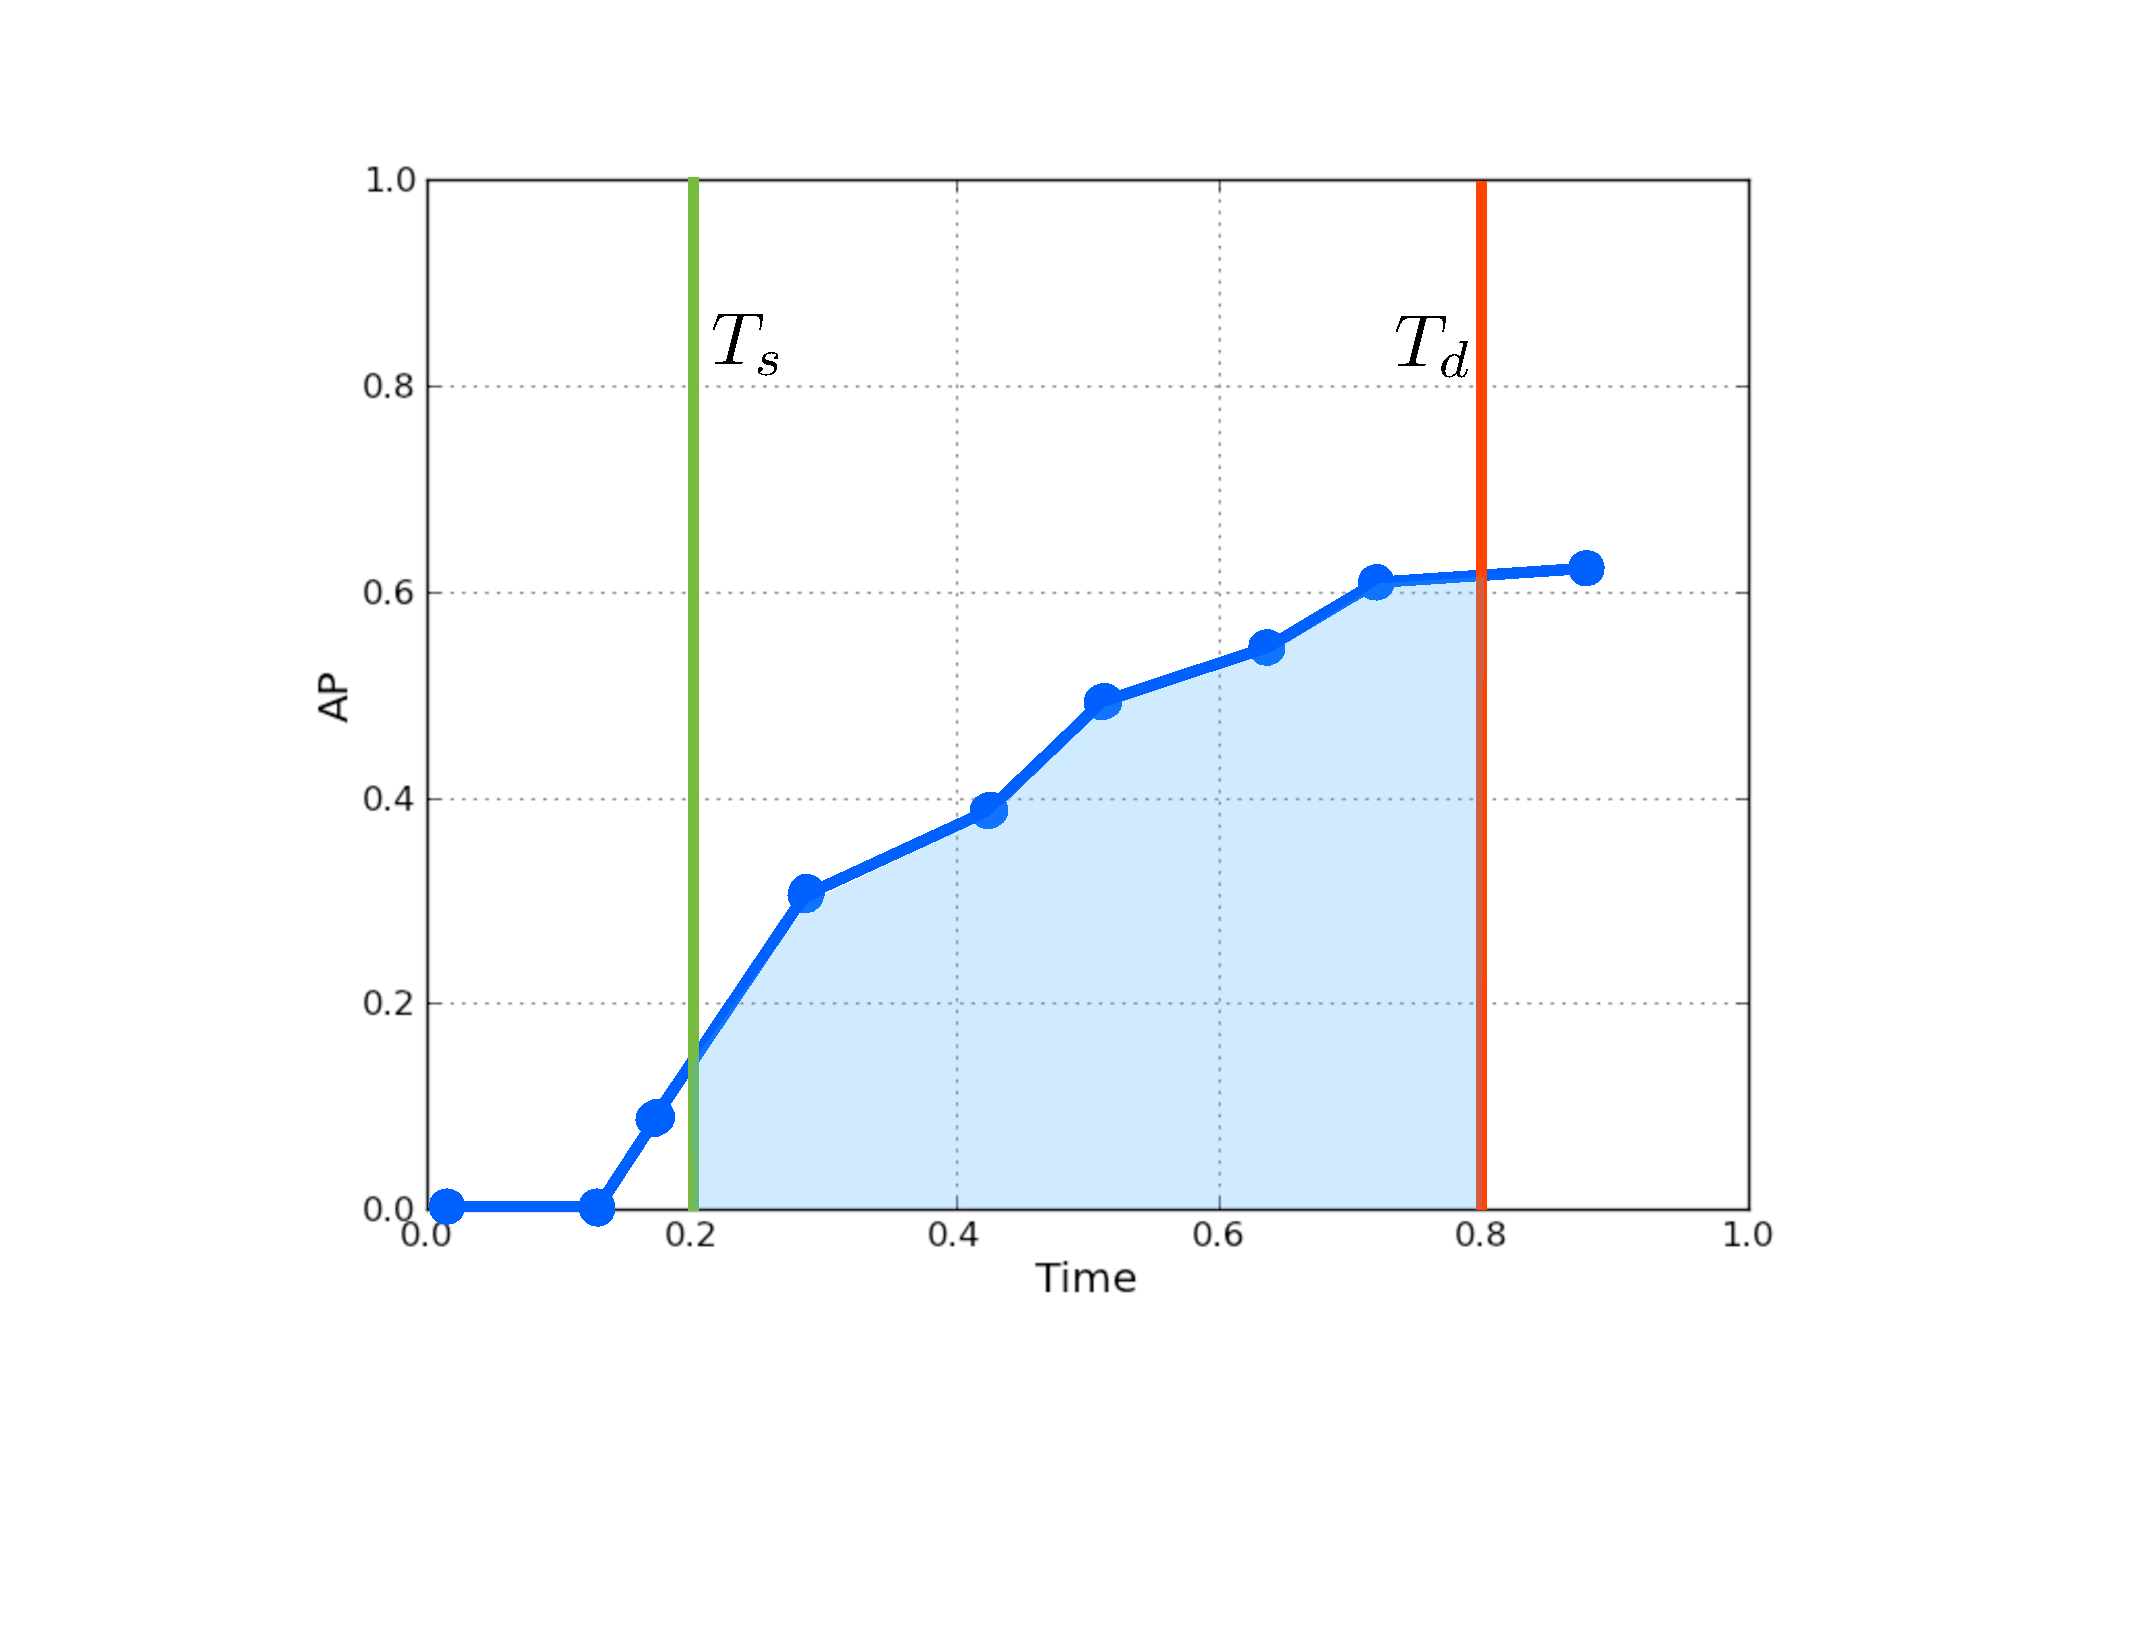
\includegraphics[width=0.56\linewidth]
    {figures/evaluation.pdf}}
  \caption{We aim for \emph{Anytime} performance within the bounds of the curve. That is, the policy should give the best possible answer at any time from start time $T_s$ to deadline $T_d$.}
  \label{fig:evaluation}
\end{figure}

To meet this goal, the evaluation metric of a policy is defined as the area under the performance vs. time curve between points $T_s$ and $T_d$ (see Figure~\ref{fig:evaluation}).
We evaluate policies by this more robust metric and not simply by the final performance at deadline time for the same reason that Average Precision is used instead of a fixed Precision vs. Recall point.

An action $a_i$ that consists of running a classifier $L_i$ returns a real-valued observation $o_i \sim P(O_i)$.
The state records the fact that $a$ has been taken by adding it to the initially empty set $\mathcal{O}$.
We refer to the current set of observations as $\mathbf{o} = \{o_i | L_i \in \mathcal{O}\}$.

We define the state $b$ of the decision process by the the distribution over class presence variables $P(\mathbf{C}) = P(C_1, \dots, C_K)$\footnote{We write $P(C_k)$ to mean $P(C_k=1)$.}, the time into episode $t$, and the set of executed actions $\mathcal{O}$ with corresponding observations $\mathbf{o}$.

A classification \emph{episode} takes an image $\mathcal{I}$ and proceeds from the initial belief state $b^0$ and action $a^0$ to the next pair $b^1$, and so on until $t$ exceeds $T_d$.
At that point, the policy is terminated and a new episode begins on a new image.

The policy's performance is determined by treating the final values of $P(\mathbf{C})$ as the set of confidence scores $\{\emph{classify}(1), \dots, \emph{classify}(K)\}$ for the multi-label classification evaluation described in \autoref{sec:problem_setting}.

For ease of reference, our notation is summarized in \autoref{tab:notation}.

\section{Selecting actions} \label{sec:value}
Optimal performance results from becoming maximally certain of the correct values $C_i$ as quickly as possible (given the setup time).
As our goal is to pick actions, we want to formulate a function $V(b,a)$ 	that assigns a value to a potential action, given the current state of the decision process.
We can then define the policy as simply
\begin{align}
\pi(b) = \argmax_{a_i \in \mathcal{A} \setminus \mathcal{O}} V(b,a_i)
\end{align}

Our system will be evaluated by some properties of the state $b$, and its performance is time-sensitive.
Accordingly, the value function should balance two terms: a function of the expected next belief state $b'$ after taking an action $a_i$, and the cost of $a_i$.
\begin{align}
V(b,a_i) = \mathbb{E}_{b' \sim P(b'|b,a_i)}[R(b')] - \lambda c(a_i|b)
\end{align}

We can be more explicit and split $b$ into its constitutents, such as the current set of observations $\mathbf{o}$ and the posterior distribution $P(\mathbf{C}|\mathbf{o})$.
Accordingly, we have considerable flexibility in definining the ``reward'' function $R(b)$.

We consider a formulation of $R(b)$ based on information gain, as is common in problems of this type \todo{cite}.
The corresponding $R: P \mapsto \mathbb{R}$ is a function on the distribution over $\mathbf{C}$.
We note that as our goal is to reduce uncertainty of $P(\mathbf{C})$, it is natural to define $R$ as the negative entropy of the distribution given the observations.
\begin{align}
V(b,a_i)
&= \mathbb{E}_{o_i \sim P(O_i|\mathbf{C},\mathbf{o})}[R(P(\mathbf{C}|\mathbf{o} \cup o_i)] - \lambda c(a_i|\mathcal{O}) \\
&= \mathbb{E}_{o_i \sim P(O_i|\mathbf{C},\mathbf{o})}[-H(\mathbf{C}|\mathbf{o} \cup o_i)] - \lambda c(a_i|\mathcal{O})
\end{align}

Keeping in mind that $ H(\mathbf{C}|\mathcal{O}) = -\sum_{\mathbf{c}} P(\mathbf{c}|\mathcal{O}) \log P(\mathbf{c}|\mathcal{O}) $ is constant w.r.t $a_i$, it is easy to show that the policy consists of picking the action that maximizes information gain of $P(\mathbf{C})$, balanced with the cost of the action:
\begin{align}
\pi(b)
&= \argmax_{a_i \in \mathcal{A} \setminus \mathcal{O}} \, \mathbb{E}_{o_i \sim P(O_i|\mathbf{C},\mathbf{o})}[-H(\mathbf{C}|\mathbf{o} \cup o_i)] + H(\mathbf{C}|\mathbf{o}) - H(\mathbf{C}|\mathbf{o}) - \lambda c(a_i|\mathcal{O}) \\
&= \argmax_{a_i \in \mathcal{A} \setminus \mathcal{O}} \, I(\mathbf{C};O_i|\mathbf{o}) - H(\mathbf{C}|\mathbf{o}) - \lambda c(a_i|\mathcal{O}) \\
&= \argmax_{a_i \in \mathcal{A} \setminus \mathcal{O}} \, I(\mathbf{C};O_i|\mathbf{o}) - \lambda c(a_i|\mathcal{O})
\end{align}

\subsection{The model of the belief state}
\begin{figure}[h!]
\centering
% \subfloat[MRF]{
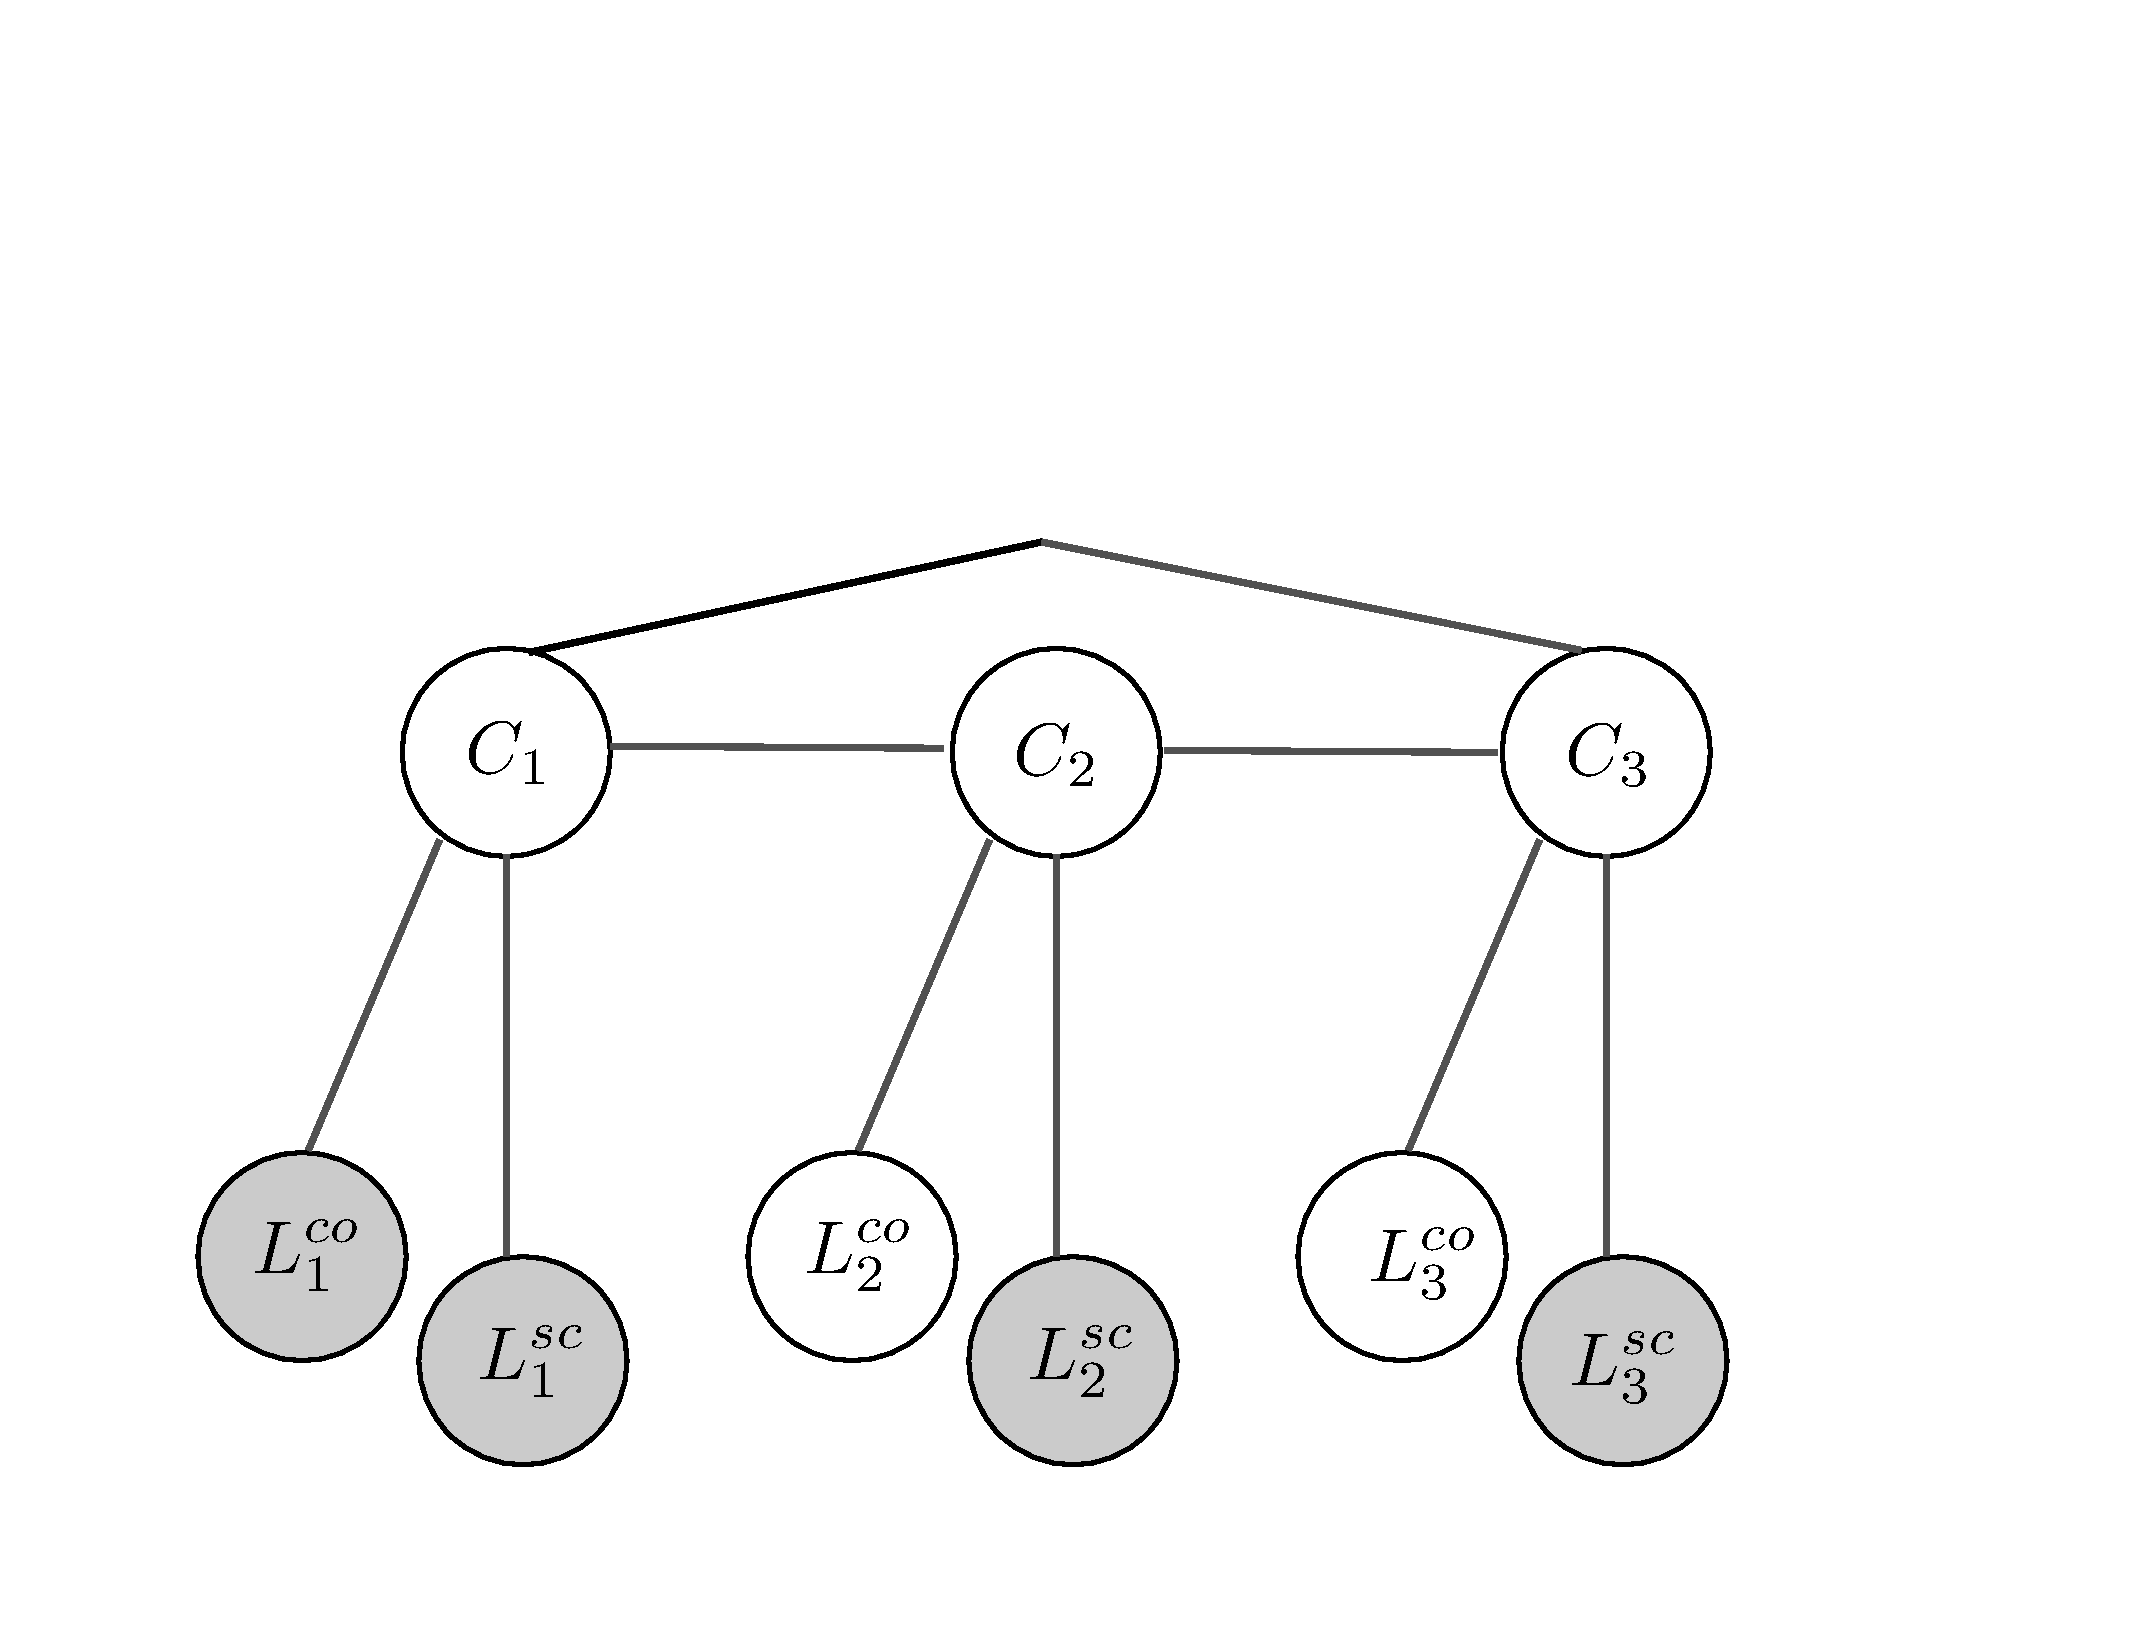
\includegraphics[width=0.56\linewidth]{figures/inf_model_mrf.pdf}
% }
% \subfloat[Local]{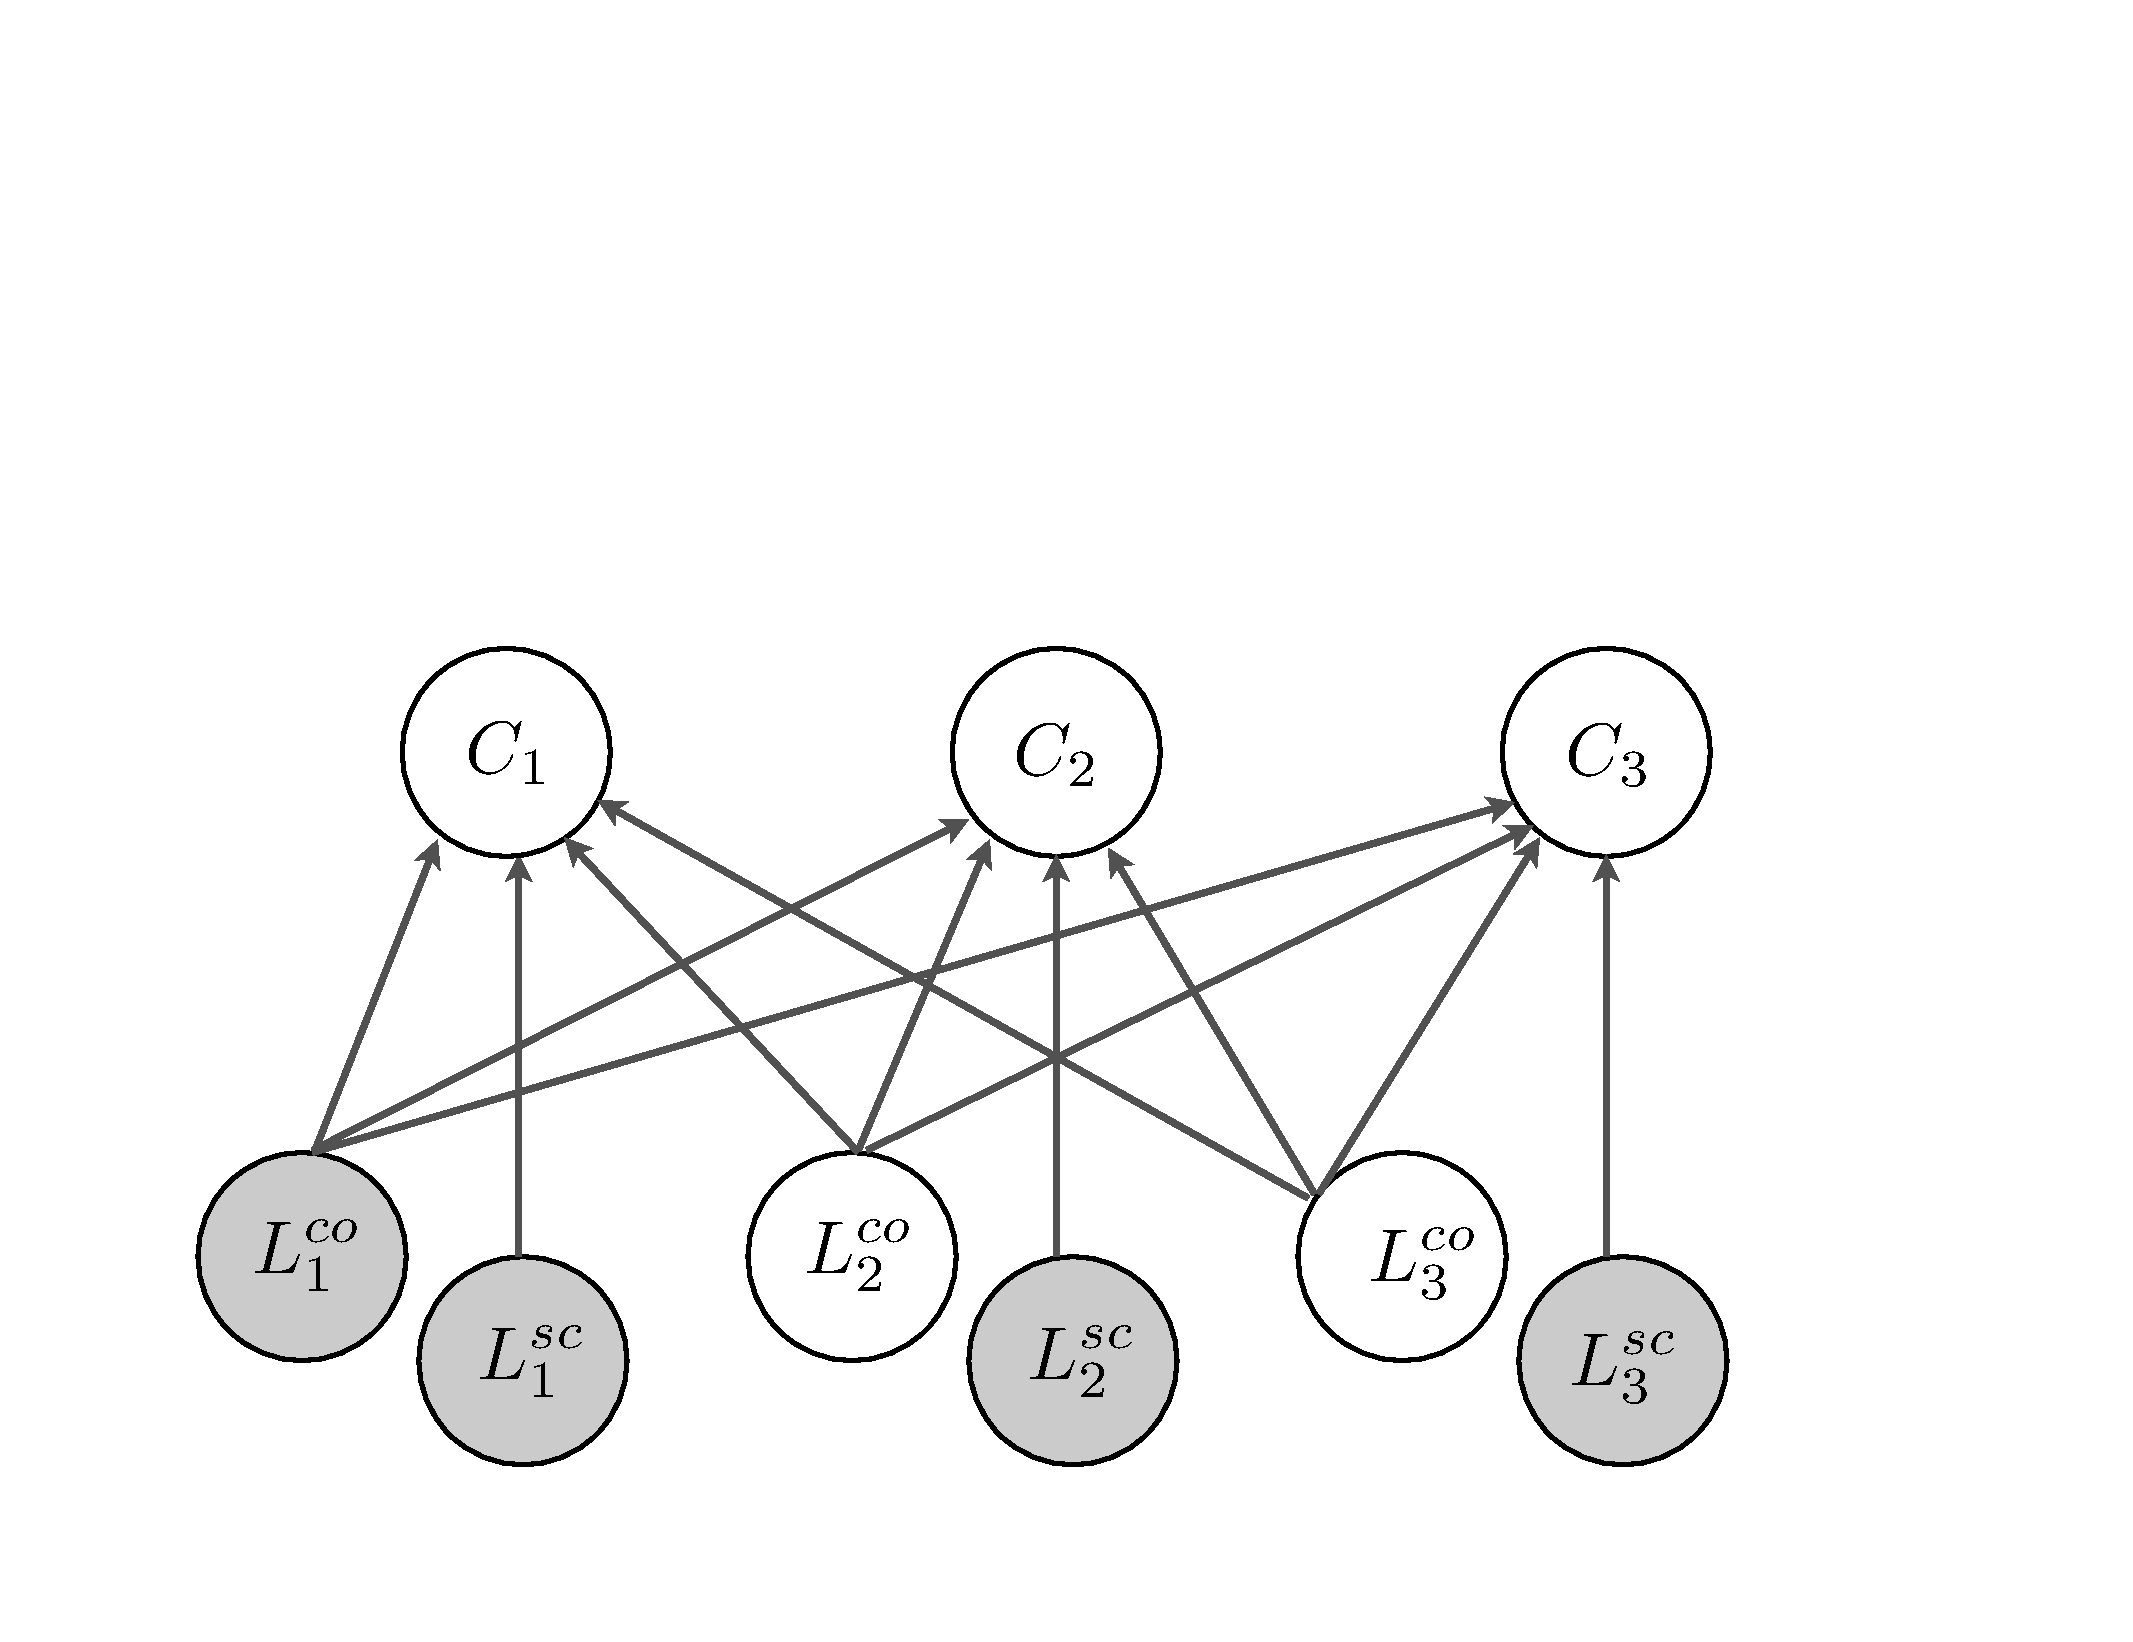
\includegraphics[width=0.46\linewidth]{figures/inf_model_loc.pdf}}
\caption{We present a point in the middle of the decision process, when some classifiers have already been observed.}
\label{fig:model}
\end{figure}

Evaluation of our policy depends on being able to efficiently compute the marginals $o_i$ and the expected information gain $I(\mathbf{C};O_i|\mathbf{o})$.
We employ a fully-connected Markov Random Field (MRF), as shown in Figure~\ref{fig:model}.
The parameters are trained on fully-observed data.
Exact inference is of course intractable in a general model of this type, and quite slow for a model of our size.
Instead, we use Loopy Belief Propagation, which provides no general convergence guarantees but has been shown to work well empirically \todo{cite}.
The implementations details are given further in \autoref{sec:implementation}.

\subsection{Submodularity} \label{sec:submodularity}
A natural question regarding our exposition so far is, why should we assume that a greedy policy would work well at all?
In fact, the problem as described has properties that here allow us to show that the greedy solution is near-optimal.

We first introduce the notion of submodularity.
A set function $f$ is submodular if, whenever $A \subseteq B \subseteq E$ and $e \in E \setminus B$ it holds that
\begin{equation}
f(A \cup {e}) - f(A) \geq f(B \cup {e}) - f(B)
\end{equation}

Additionally, $f$ is called monotone if whenever $A \subseteq B$ it holds that $f(A) \leq f(B)$.
Nemhauser~\cite{Nemhauser1978} famously showed that a greedy algorithm applied to maximizing submodular monotone functions with $f(\emptyset)=0$ will obtain at least a $(1-1/e)$ fraction of the optimal solution.

Krause and Guestrin~\cite{Krause2005a} showed that the result applies to the problem of selecting a set of observations, such as in a sensor network, which maximally reduces uncertainty.
Specifically, they showed that if the function to be maximized by selecting observations $S$ is information gain of latent variables $U$ in a graphical model such that variables in $S$ are independent given $U$, the greedy selection algorithm gives the same near-optimal bound as  ~\cite{Nemhauser1978}, and that no polynomial-time algorithm can be guaranteed to give a better bound, unless $P \neq NP$.

\todo{adaptive submodularity \cite{Golovin2011}}

\subsection{Policy parametrization and more reward functions}
\todo{here introduce the view of learning parameters given the observed rewards}

Let's say that given deadline $T_d$ and some image, the policy had time to take $J$ actions.
The total expected reward of a policy $\pi$ is then defined as the sum of rewards
\begin{equation}
\mathbb{E}_\pi[\sum_{j=0}^J R(b_j)]
\end{equation}

The reward function does not necessarily have to be related to the evaluation of the system.

\subsubsection{Slope of performance vs. time}
\begin{figure}[htb]
  \centering
  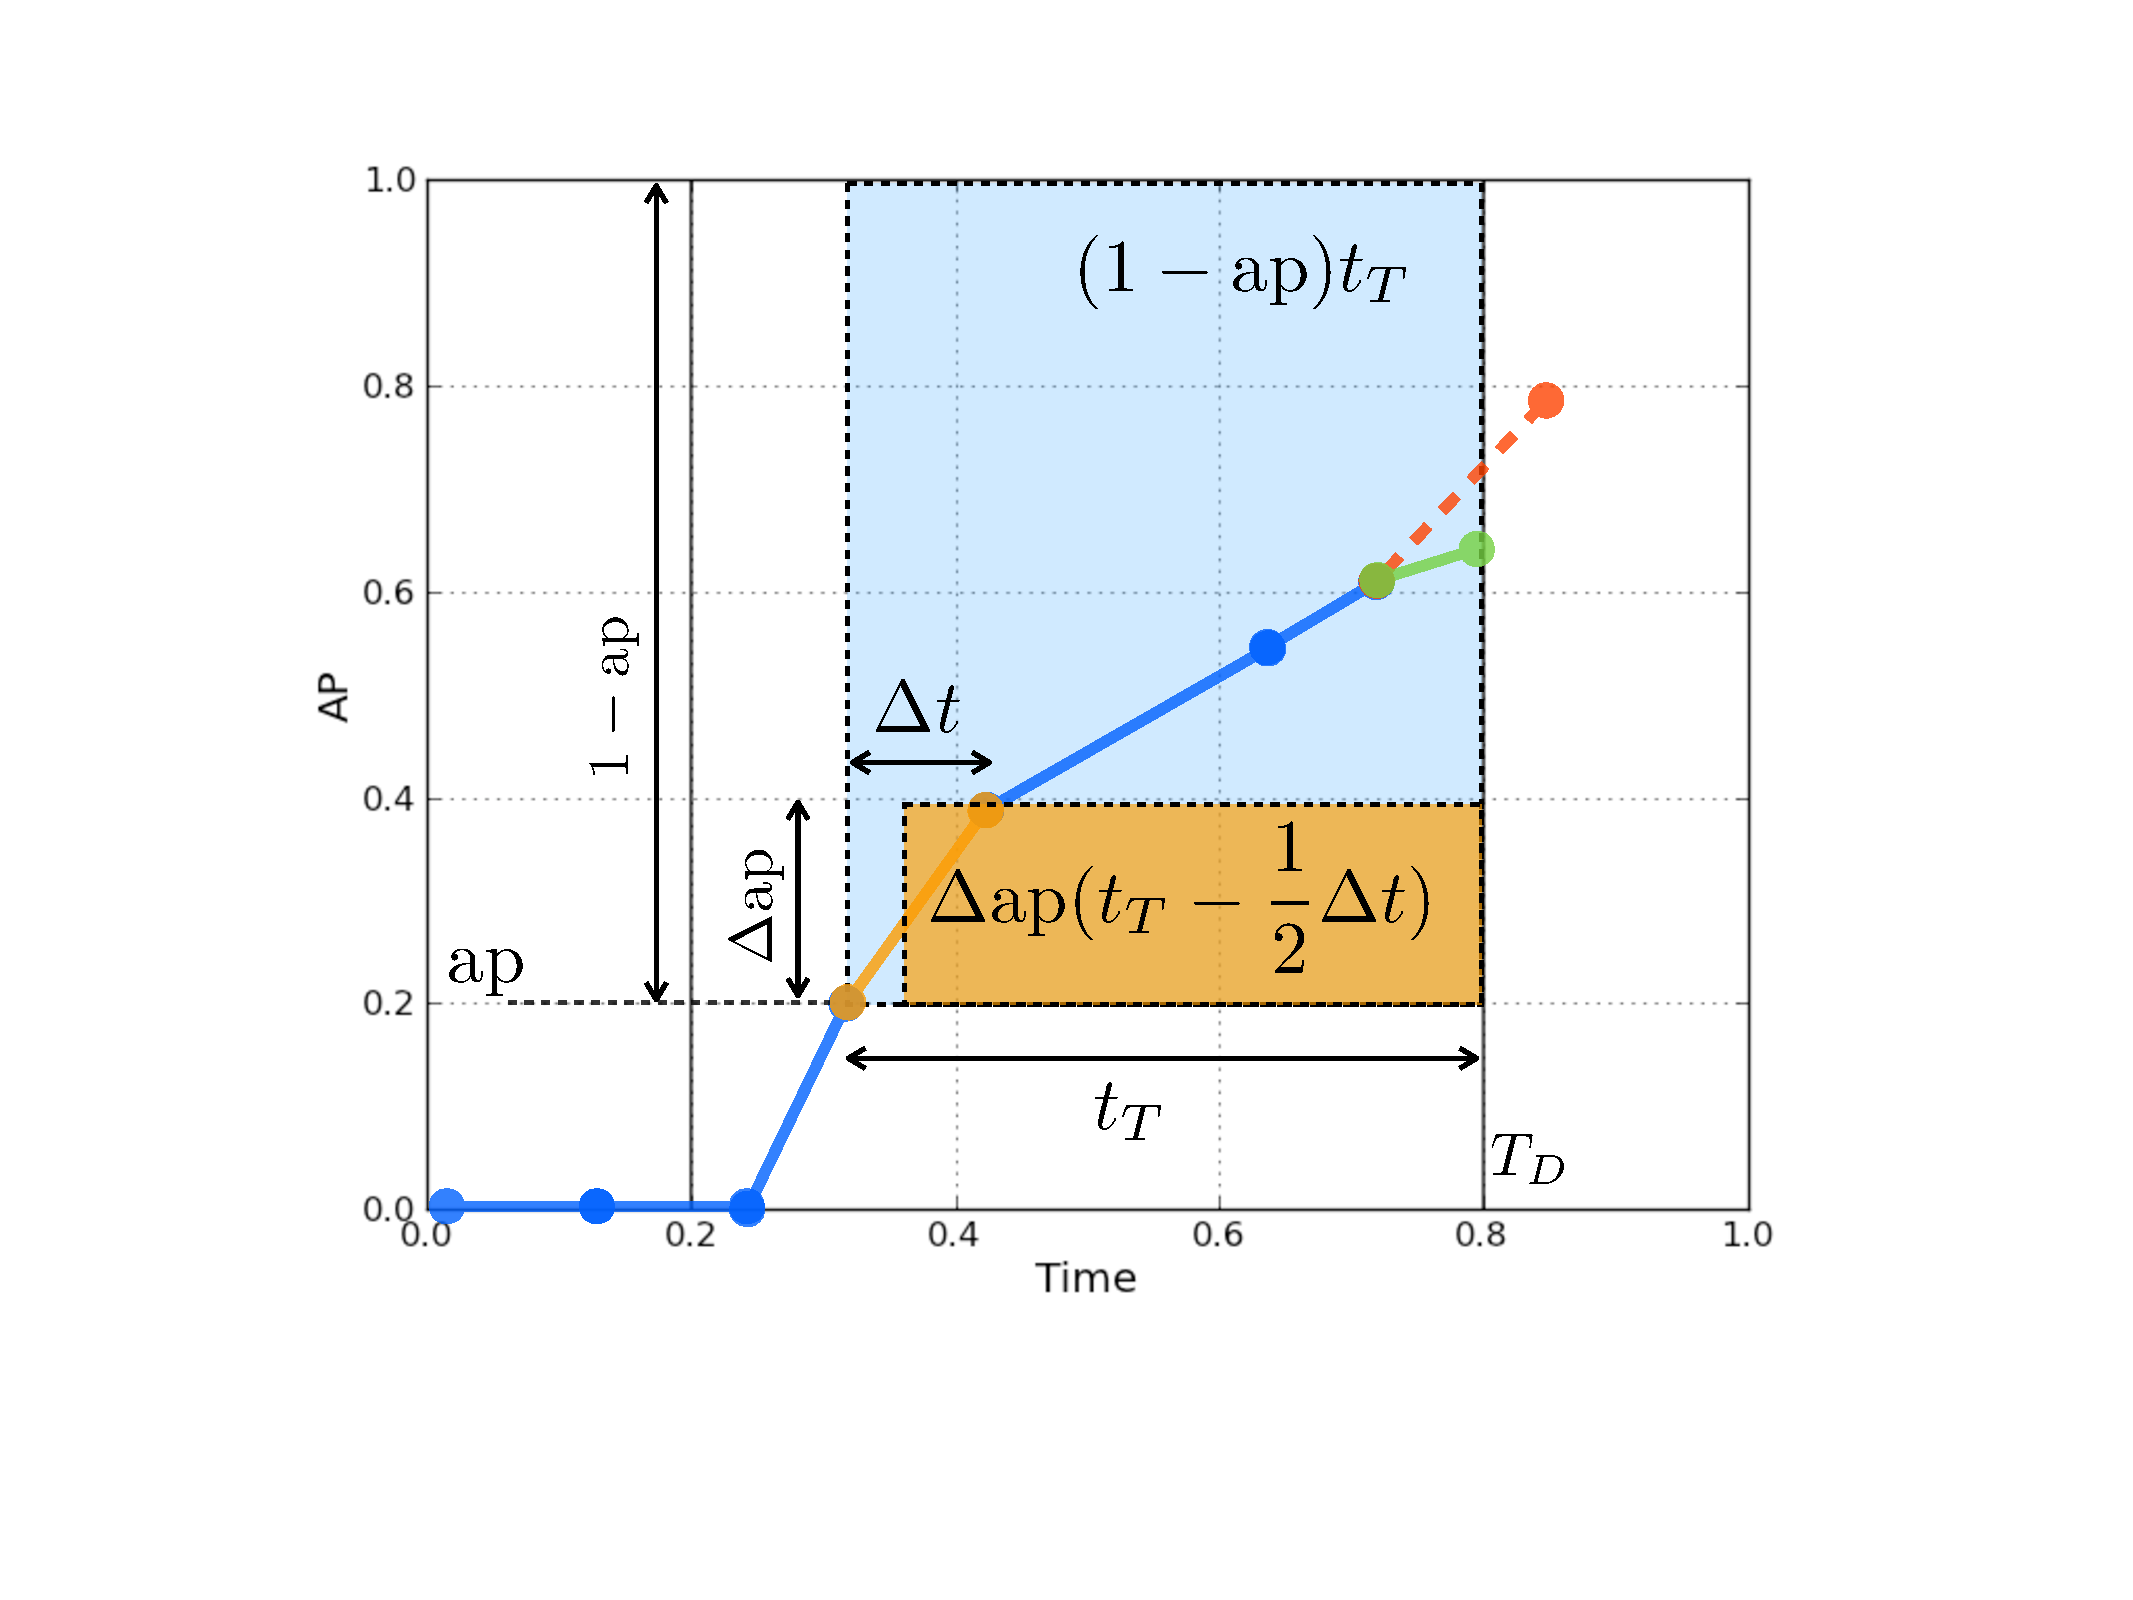
\includegraphics[width=0.56\linewidth]{figures/apvst_expl.pdf}
  \caption{A per-action greedy value function that corresponds to the maximization of our objective function is the area of the horizontal slice under the curve due to the action. The figure shows this analysis for the action highlighted in orange.}
  \label{fig:rewards}
\end{figure}

Remembering that the final evaluation of a policy consists of the area under the performance vs. time curve, we formulate per-action rewards such that their addition results in precisely this quantity.
Specifically, as shown in Figure~\ref{fig:rewards}, we define the reward of an action as
\begin{equation}\label{eq:advanced}
\Delta AP (t_T-\Delta t)
\end{equation}
where $t_T$ is the time left until deadline, and $\Delta t$ and $\Delta AP$ are the time taken and AP change produced by the action.

The equation breaks down into a term to maximize, $\Delta AP t_T$, and a term to minimize, $\Delta AP \Delta t$.
This agrees with the intuition that to capture the most area under the curve, the slope needs to be maximized at each point.
Additionally, the equation shows that if $\Delta t$ exceeds $t_T$, the value of taking the action is negative.

At each step, we want to pick the action that maximizes the expected rewards until the end of the episode.
We therefore define our policy as
\begin{equation}
\pi(b) = \argmax_{a \in \mathcal{A} \setminus \mathcal{O}} \theta^\top \phi(b,a)
\end{equation}

Learning this accurately is the domain of Reinforcement Learning research, and is generally intractable for large-scale POMDPs.

First, we seek to maximize the expected next-stage reward, and manually construct a value function such that picking the action with maximal value achieves this.
Next, we note that the manually constructed value function can be represented as a scalar product of a parameter vector with a featurization of the belief state; we learn the weights by regression to the actual next-stage reward from running many episodes.
Lastly, we use a reinforcement learning technique to learn the weights such that the expected rewards over the whole episode are maximized.

\subsubsection{Learning the greedy policy}
We note that we can represent the one-step greedy policy value function as a scalar product 

\subsubsection{Learning the proper policy}
\note{I'm considering two options here: (1) log-linear representation and policy gradient algorithm; (2) least-squares policy iteration.}

\paragraph{Policy gradient algorithm}
We redefine our policy as picking the mode of a log-linear parametrized distribution:
\begin{equation}
P(a|b;\theta) = \frac{\exp(\theta^T \phi(b,a))}{\sum_{a' \in \mathcal{A}} \exp(\theta^T \phi(b,a')}
\end{equation}

Basically stochastic gradient ascent on the estimate of the reward accrued by an episode.

This approach has been shown to scale to large problems in \cite{Branavan2009}, although it has been proven to converge only to local maxima and only for MDPs \cite{Sutton2000}.

\note{Does the constraint that no action is taken more than once affect this algorithm?}

\paragraph{Least-squares Policy Iteration}
An efficient form of temporal-difference learning used in \cite{Kwok2004}.
Policy remains parameterized as it was.

\section{Implementation Details and Evaluation} \label{sec:implementation}
We use FastInf \cite{Jaimovich2010} for learning and inference in our MRF model.
The real-valued classifier responses $o_i$ are discretized into data-dependent bins for efficiency.

\section{Evaluation} \label{sec:evaluation}
- show that the greedy policy works better than random and better than fixed-order

- show that the reinforcement learning policy works better than greedy, at least for the non-infogain rewards.

\subsection{Classification}

\subsection{Detection}
We also evaluate using the task of detection (see \autoref{sec:problem}).


\bibliographystyle{splncs}
\bibliography{sergeyk-bibtex}

\end{document}
